\section{CUESTIONES}
\subsection{El concepto de juego. Elementos y clasificación de los juegos.}
\subsection{El algoritmo minmax. Componentes y funcionamiento.}
\subsection{Modelos de representación del conocimiento.}
\subsection{Modelos de conocimiento heredable. Herencia.}
\subsection{Paradigmas de aprendizaje.}
\subsection{Aprendizaje inductivo. Empleo de árboles de decisión en aprendizaje inductivo.}
\pagebreak
\section{RESPUESTAS}
\subsection{El concepto de juego. Elementos y clasificación de los juegos.}
		    \centering 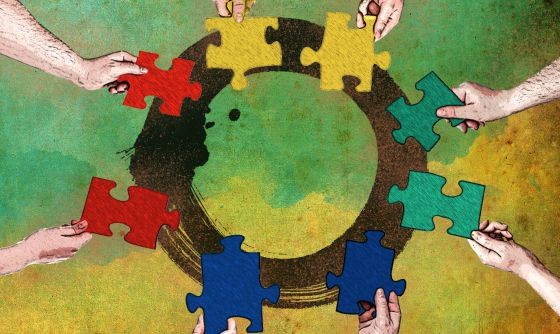
\includegraphics[width=0.9\textwidth]{juegos.jpg}
Un juego es cualquier situación de decisión con \textbf{varios agentes} (llamados jugadores) gobernada por un \textbf{conjunto de reglas} y con un resultado bien definido, caracterizada porque \textbf{ninguno de los jugadores con su sola actuación puede determinar el resultado} (independencia estratégica).
Lo que caracteriza a un juego particular es el \textbf{número de jugadores}, la \textbf{información con que cuentan los jugadores} (perfecta o imperfecta), la \textbf{existencia o no de movimientos de azar}, el \textbf{orden de actuación de los jugadores}, los \textbf{repartos de beneficios} (que determinan si se trata de juegos de suma nula o no nula) y la \textbf{existencia o no de pagos colaterales} (equilibrio de Nash).
